\newpage
\section{Registro ore}
Nei seguenti paragrafi verrà spiegato come il gruppo intende dividere l'impegno dei ruoli nei sei diversi periodi di sviluppo del software. Successivamente verranno inserite le ore di investimento complessive nel gruppo. 
All'ultimo paragrafo, verrà mostrato un riassunto con il totale del peso dei vari ruoli nell'intero progetto.

\subsection{Periodo di Analisi dei Requisiti}
Il primo periodo è l'\AdR. Esso non è rendicontabile ai fini di calcolo del preventivo, poichè non è da considerarsi a carico del \textit{Proponente}. Le ore totali sono suddivise come segue:

\begin{table}[H]
	\begin{center}
		\begin{tabular}{|c|c|c|}
			\hline
			\textbf{Ruolo}	& \textbf{Ore}	& \textbf{Ore rendicontabili} \\
			\hline
			\Res	&	38	&  0 \\
			\hline
			\Amm	&	11	&  0 \\
			\hline
			\Ana	&	79	&  0 \\
			\hline
			\Ver	&	61	&  0 \\
			\hline
			\textbf{Totale} & \textbf{189} & \textbf{0} \\
			\hline
		\end{tabular}
	\end{center}
	\caption{Ore per ruolo, periodo di Analisi dei Requisiti}
\end{table}

L'incidenza di tali ore determina in percentuale, come mostrato di seguito:
\begin{figure}[H]
	\centering
	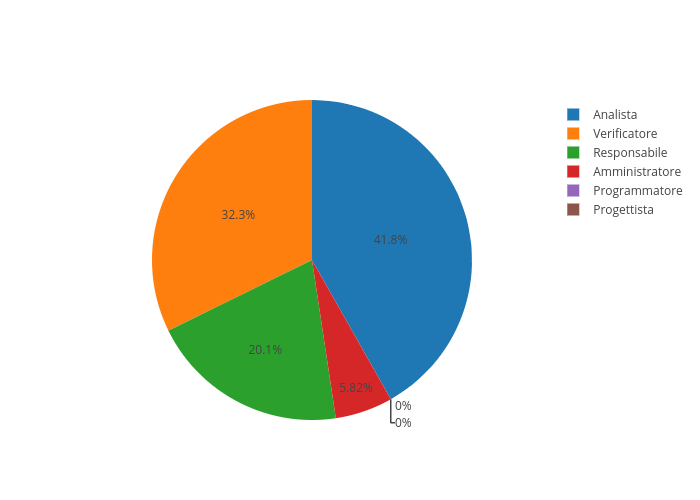
\includegraphics[scale=0.6]{img/AnalisiRequisiti.png}
	\caption{Incidenza ore per ruolo, periodo di Analisi dei Requisiti}
\end{figure}

\subsection{Periodo di Analisi dei Requisiti Dettagliata}
La seconda porzione di \AdR, da svolgersi dopo la \RR, è l'Analisi dei Requisiti Dettagliata. Come per il precedente, esso è da considerarsi parte dell'investimento intrapreso e quindi, non è rendicontabile ai fini del calcolo del preventivo. Le ore totali sono suddivise come segue:

\begin{table}[H]
	\begin{center}
		\begin{tabular}{|c|c|c|}
			\hline
			\textbf{Ruolo}	& \textbf{Ore}	& \textbf{Ore rendicontabili} \\
			\hline
			\Res	&   4 	&  0  \\
			\hline
			\Amm	&   1	&  0	\\
			\hline
			\Ana	&   5	&  0	\\
			\hline
			\Ver	&   5	&  0	\\
			\hline
			\textbf{Totale} & \textbf{15} & \textbf{0} \\
			\hline
		\end{tabular}
	\end{center}
	\caption{Ore per ruolo, periodo di Analisi dei Requisiti Dettagliata}
\end{table}

L'incidenza di tali ore determina in percentuale, come mostrato di seguito:
\begin{figure}[H]
	\centering
	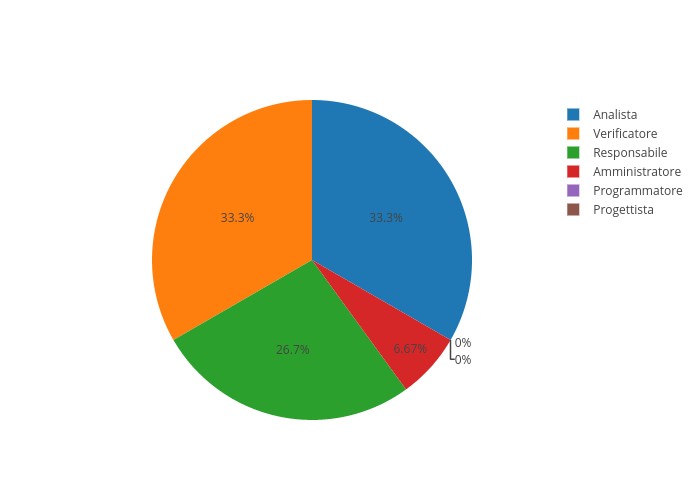
\includegraphics[scale=0.6]{img/AnalisiRequisitiDettaglio.png}
	\caption{Incidenza ore per ruolo, periodo di Analisi dei Requisiti Dettagliata}
\end{figure}

\subsection{Periodo di Progettazione Architetturale}
Lo sviluppo procede con la Progettazione Architetturale. Le ore totali sono suddivise come segue:

\begin{table}[H]
	\begin{center}
		\begin{tabular}{|c|c|c|}
			\hline
			\textbf{Ruolo}	& \textbf{Ore}	& \textbf{Ore rendicontabili} \\
			\hline
			\Res	&	5	&	5	\\
			\hline
			\Amm	&	5	&	5	\\
			\hline
			\Prog   &	138   &	138	\\
			\hline
			\Ver	&	52	&	52	\\
			\hline
			\textbf{Totale} & \textbf{200} & \textbf{200} \\
			\hline
		\end{tabular}
	\end{center}
	\caption{Ore per ruolo, periodo di Progettazione Architetturale}
\end{table}

L'incidenza di tali ore determina in percentuale, come mostrato di seguito:
\begin{figure}[H]
	\centering
	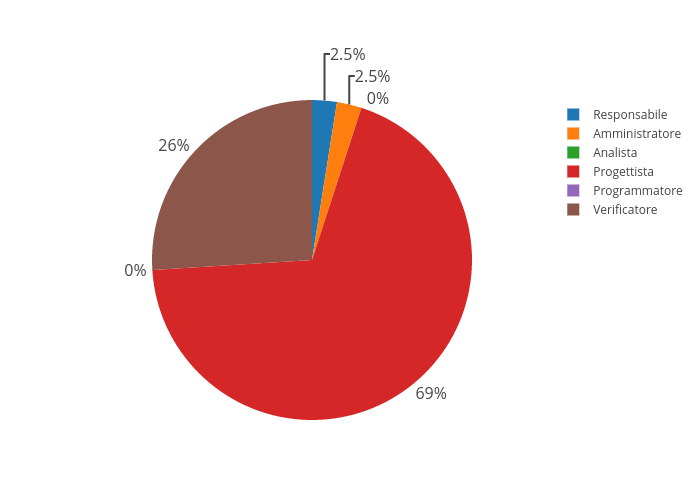
\includegraphics[scale=0.6]{img/ProgettazioneArchitetturale.png}
	\caption{Incidenza ore per ruolo, periodo di Progettazione Architetturale}
\end{figure}

\subsection{Periodo di Progettazione Architetturale Dettagliata}
Il terzo periodo è la Progettazione Architetturale Dettagliata. Le ore totali sono suddivise come segue:

\begin{table}[H]
	\begin{center}
		\begin{tabular}{|c|c|c|}
			\hline
			\textbf{Ruolo}	& \textbf{Ore}	& \textbf{Ore rendicontabili} \\
			\hline
			\Res	&	5	&	5 \\
			\hline
			\Amm	&	6	&	6	\\
			\hline
			\Prog   &	72   &	72	\\
			\hline
			\Ver	&	35	&	35	\\
			\hline
			\textbf{Totale} & \textbf{118} & \textbf{118} \\
			\hline
		\end{tabular}
	\end{center}
	\caption{Ore per ruolo, periodo di Progettazione Architetturale Dettagliata}
\end{table}

L'incidenza di tali ore determina in percentuale, come mostrato di seguito:
\begin{figure}[H]
	\centering
	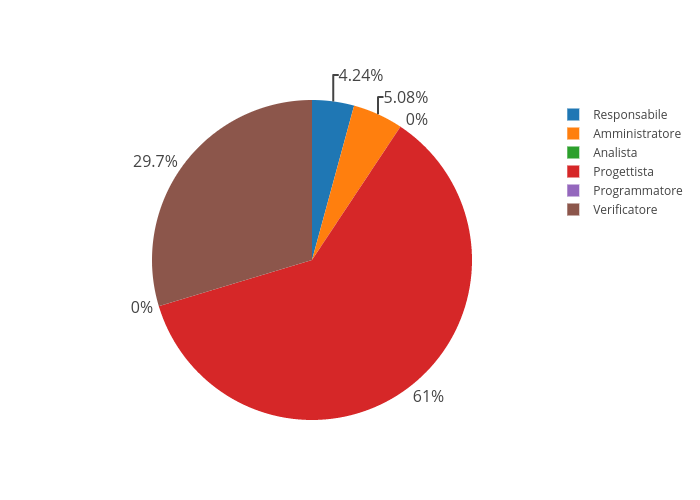
\includegraphics[scale=0.6]{img/ProgettazioneDettaglio.png}
	\caption{Incidenza ore per ruolo, periodo di Progettazione Architetturale Dettagliata}
\end{figure}

\subsection{Periodo di Codifica}
Il penultimo periodo è la Codifica. Le ore totali sono suddivise come segue:

\begin{table}[H]
	\begin{center}
		\begin{tabular}{|c|c|c|}
			\hline
			\textbf{Ruolo}	& \textbf{Ore}	& \textbf{Ore rendicontabili} \\
			\hline
			\Res	&	6	&	6	\\
			\hline
			\Amm	&	3	&	3	\\
			\hline
			\Progr   &	143   &	143	\\
			\hline
			\Ver	&	61	&	61	\\
			\hline
			\textbf{Totale} & \textbf{213} & \textbf{213} \\
			\hline
		\end{tabular}
	\end{center}
	\caption{Ore per ruolo, periodo di Codifica}
\end{table}

L'incidenza di tali ore determina in percentuale, come mostrato di seguito:
\begin{figure}[H]
	\centering
	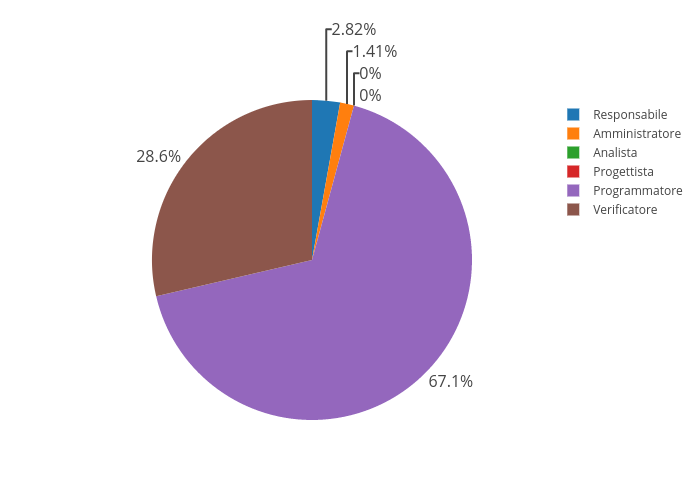
\includegraphics[scale=0.6]{img/Codifica.png}
	\caption{Incidenza ore per ruolo, periodo di Codifica}
\end{figure}

\subsection{Periodo di Verifica e Validazione}
L'ultimo periodo è la Verifica e Validazione del prodotto sviluppato. Le ore totali sono suddivise come segue:

\begin{table}[H]
	\begin{center}
		\begin{tabular}{|c|c|c|}
			\hline
			\textbf{Ruolo}	& \textbf{Ore}	& \textbf{Ore rendicontabili} \\
			\hline
			\Res	&	3  &	3	\\
			\hline
			\Amm	&	3  &	3	\\
			\hline
			\Prog   &	15  &	15	\\
			\hline
			\Ver	&	78	&	78	\\
			\hline
			\textbf{Totale} & \textbf{99} & \textbf{99} \\
			\hline
		\end{tabular}
	\end{center}
	\caption{Ore per ruolo, periodo di Verifica e Validazione}
\end{table}

L'incidenza di tali ore determina in percentuale, come mostrato di seguito:
\begin{figure}[H]
	\centering
	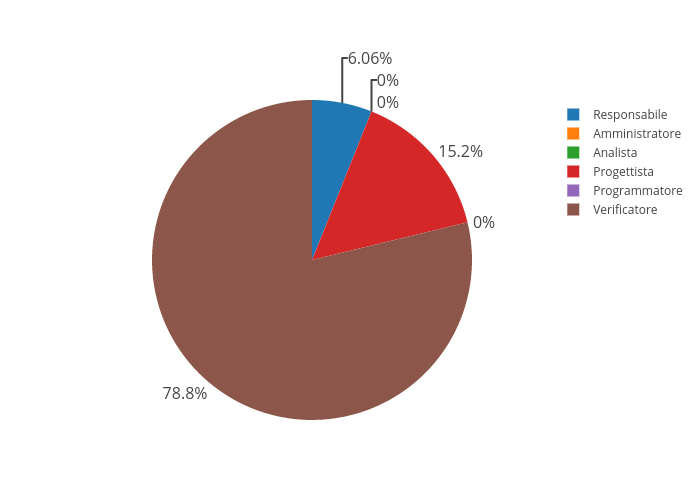
\includegraphics[scale=0.6]{img/Validazione.png}
	\caption{Suddivisione ore per ruolo, periodo di Verifica e Validazione}
\end{figure}

\subsection{Ore di investimento}
La quota di investimento comprende le ore necessarie ad apprendere le tecnologie richieste per la realizzazione del progetto. Queste ore esulano dalle ore di \textit{Analisi dei Requisiti} e non sono a carico del \textit{Proponente}. L'investimento delle ore per auto formazione sulle tecnologie necessarie allo svolgimento del progetto si è concentrato principalmente nel periodo di progettazione, come mostrato di seguito.
\begin{figure}
	\centering
	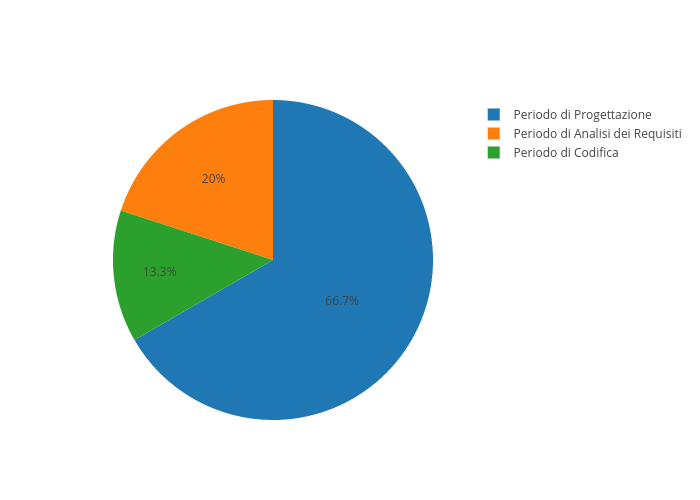
\includegraphics[scale=0.6]{img/ore_investimento_periodi}
	\caption{Ripartizione ore investimento}
	\label{fig:oreinvestimentoperiodi}
\end{figure}
Le ore complessive dedicate dai membri del gruppo sono 220 e riguardano auto formazione individuale sulle tecnologie necessarie e di indispensabile conoscenza da parte di tutti i membri del gruppo. Tutti i membri del gruppo, all'inizio del periodo di progettazione hanno affermato di avere buona padronanza delle seguenti tecnologie:
\begin{itemize}
	\item HTML5\ped{G};
	\item CCS3\ped{G};
	\item Java\ped{G};
	\item MySQL\ped{G}.
\end{itemize}
Le ore di auto formazione quindi, si sono concentrate sulle tecnologie rimanenti, ovvero:
\begin{itemize}
	\item Bootstrap 3\ped{G};
	\item Jolie\ped{G};
	\item Javascrpipt\ped{G} e i relativi framework:
	\begin{itemize}
		\item Angular 2\ped{G};
		\item Meteor JS\ped{G};
		\item Jquery\ped{G}.
	\end{itemize}
	\item Leonardo\ped{G}.
\end{itemize}
Si segnala che un membro ha affermato di conoscere il framework \textit{Bootstrap 3\ped{G}}, per cui tralascerà l'auto formazione su tale tecnologia.

Di seguito sono riportate le ore che ogni membro ha dedicato all'auto formazione relativa alle tecnologie:

\begin{table}[H]
	\begin{center}
		\begin{tabular}{|c|c|}
			\hline
			\textbf{Ruolo}	& \textbf{Ore dedicate}  \\
			\hline
			\MC	&	33		\\
			\hline
			\DAN	&	34	\\
			\hline
			\AN	&	34		\\
			\hline
			\AS	&	31		\\
			\hline
			\NS	&	33		\\
			\hline
			\DS	&	32		\\
			\hline
			\textbf{Totale} & \textbf{197}  \\
			\hline
		\end{tabular}
	\end{center}
	\caption{Ore per auto formazione sulle tecnologie}
\end{table}


\subsection{Riepilogo}
Le ore totali del necessarie allo sviluppo sono 837 di cui, scorporando la fase di Analisi dei Requisiti, 630 remunerabili. Complessivamente le ore sono suddivise come segue:

\begin{table}[H]
	\begin{center}
		\begin{tabular}{|c|c|c|}
			\hline
			\textbf{Ruolo}	& \textbf{Ore complessive} & \textbf{Ore rendicontabili} \\
			\hline
			\Res	&	61	&	19	\\
			\hline
			\Amm	&	29	&	17	\\
			\hline
			\Ana	&	84	&	0	\\
			\hline
			\Prog	&	225	&	225	\\
			\hline
			\Progr	&	143	&	143	\\
			\hline
			\Ver	&	292	&	226	\\
			\hline
			\textbf{Totale} & \textbf{834} & \textbf{630} \\
			\hline
		\end{tabular}
	\end{center}
	\caption{Ore per ruolo, Riepilogo}
\end{table}

L'incidenza di tali ore incide in percentuale, come mostrato di seguito, prima complessive e poi remunerative:
\begin{figure}[H]
	\centering
	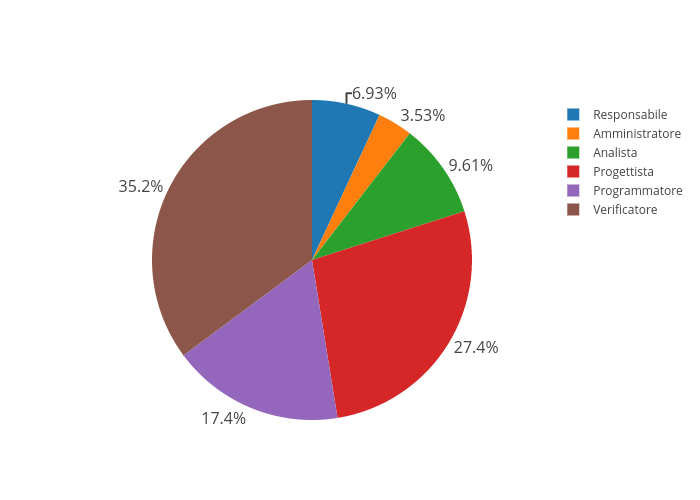
\includegraphics[scale=0.6]{img/OreTotali.png}
	\caption{Suddivisione ore per ruolo, riepilogo totale}
\end{figure}
\begin{figure}[H]
	\centering
	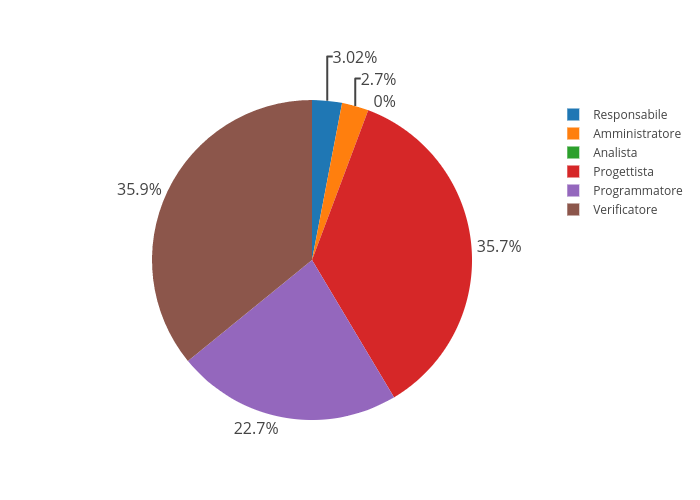
\includegraphics[scale=0.6]{img/OreRendicontabili.png}
	\caption{Suddivisione ore per ruolo, riepilogo ore remunerabili}
\end{figure}

